\section{Forschungsbeispiel}
\label{sec:Forschungsbeispiel}

Im Rahmen dieser Ausarbeitung sollen die Möglichkeiten und Grenzen selbststeuernder 
Prozesse in der Produktionslogistik untersucht werden. Die Untersuchung soll hierbei 
anhand eines Forschungsprojektes des Sonderforschungsbereichs 637 „Selbststeuerung 
logistischer Prozesse – Ein Paradigmenwechsel und seine Grenzen“ der Universität 
Bremen durchgeführt werden. Der Sonderforschungsbereich befasst sich mit der Frage, 
auf welche Weise sich Modelle, Methoden und Werkzeuge logistischer Prozesse abändern 
lassen, um eine dezentrale Selbststeuerung zu ermöglichen.

Bei dem zu untersuchenden Forschungsprojekt handelt es sich um eine Demonstrationsplattform, 
die die vom Sonderforschungsbereich erarbeiteten Selbststeuerungskonzepte anschaulich 
darstellen soll. Die Demonstrationsplattform bildet ein Produktionsszenario für die Montage 
von PKW-Rücklichtern ab. Der Montageprozess ermöglicht hierbei die Fertigung verschiedener 
Produktvarianten der PKW-Rücklichter. Weiterhin können innerhalb des Montageprozesses verschiedene 
Montagestationen flexibel durchlaufen werden. In den Produktionsprozess sind hierbei verschiedene 
Methoden der Selbststeuerung implementiert. \abbildung{Montagestation} zeigt die einzelnen Montagestationen der Demonstrationsplattform.

\begin{figure}[htb] 
\centering
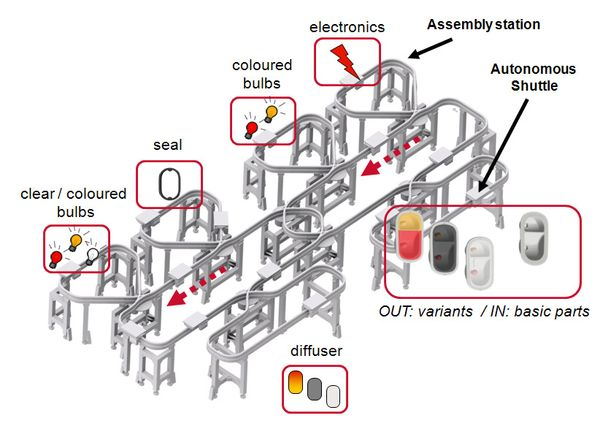
\includegraphics[width=1.0\textwidth]{Montage.jpg}
\caption[Montagestation]{Montagestationen der Demonstrationsplattform\protect\footnotemark}
\label{fig:Montagestation}
\end{figure}
\footnotetext{entnommen aus \citet[S.~xx]{xx}}

Die Demonstrationsplattform besteht aus einem Einschienensystem, auf dem sich mehrere 
Transportplattformen, sogenannte Shuttle, autonom bewegen können. Die Shuttle transportieren 
die Rücklichter einzeln durch das Montagesystem. Zu Beginn des Montageprozesses wird ein 
Reflektor-Gussteil, welcher das Ausgangsbauteil der Montage darstellt, auf dem Shuttle 
angebracht. In jedes dieser Reflektor-Gussteil wurde dabei ein RFID-Transponder integriert, 
welcher die Eindeutige Identifikation des Bauteils über den gesamten Montageprozess hinweg ermöglicht.
Im Verlauf des Montageprozesses wird das Ausgangsbauteil an verschiedenen Montagestationen um die 
Komponenten Kabelbaum, Leuchtmittel, Dichtung und Blende erweitert. Die Reihenfolge, in der die 
einzelnen Komponenten an den Reflektor angebracht werden können, ist dabei flexibel. Es müssen 
jedoch bestimmte Abhängigkeiten eingehalten werden. So müssen beispielsweise Leuchtmittel und 
Dichtung vor der Blende montiert werden. Der Kabelbaum kann hingegen zu jeder Zeit an dem Reflektor angebracht werden.

\begin{figure}[htb] 
\centering
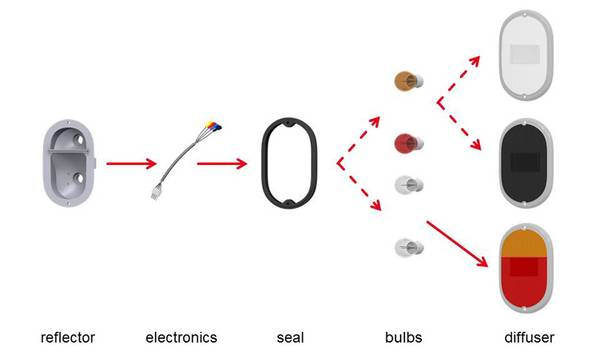
\includegraphics[width=1.0\textwidth]{Variantenkorridor.jpg}
\caption[Variantenkorridor]{Variantenkorridor\protect\footnotemark}
\label{fig:Variantenkorridor}
\end{figure}
\footnotetext{entnommen aus \citet[S.~xx]{XX}}

